\documentclass[class=article, crop=false, 12pt]{standalone}
\usepackage[subpreambles=true]{standalone}
\usepackage{../.common/common}


\author{Tony Shing}
%\pretitle{Supplementary}

\topic{Note 2A (Math for Physics)}
\title{Multivariable Calculus}

\version{2025} % leave blank for omitting

\begin{document}

\maketitle

\begin{overview}
    \begin{itemize}
        \item Comparison between single variable functions \& multivariable functions
        \item Partial differentiation (on scalar function)
        \item Multiple integral (on scalar function)
    \end{itemize}
\end{overview}



% content begins here
% Section %%%%%%%%%%%%%%%%%%%%%%%%%%%%%%%%%%%%%%%%%%%%%%%%%%%%
\section{Functions with Multiple Variables}

To well-define a function $f(x)$ in advanced mathematics,
we actually need to specify the function's \bf{domain} and \bf{image}.\\

\begin{itemize}
    \item Domain = The set of values that be substitute into $x$.
    \item Image = The set of all possible output of $f(x)$. 
\end{itemize}

E.g. Formal notation in math text to define $f(x) = \inv{|x|}$:
\aleq{
    f\colon \tkn{domain}{\cul[red]{\mathbb{R}}} & \longrightarrow \tkn{image}{\cul[blue]{\mathbb{R}^+}} \\
  x & \longmapsto \inv{|x|}
}
\addArrow[red]{domain}{(-10ex,-4ex)}{Domain}{(0,-1ex)}
\addArrow[blue]{image}{(10ex,-4ex)}{Image}{(0,-1ex)}

We can classify functions by whether their domain/image are made of single number / tuple of numbers.



%%%%%%%%%%%%%%
\subsection{Single Variable Scalar Function}

They are the functions that you have already learnt.

\begin{itemize}
    \item Domain = A set of single number
    \item Image = A set of single number 
\end{itemize}

For example, 
\aleq{
    f(x) = \sqrt{x-1} \qquad \Rightarrow \qquad 
    \bcase{
        \text{\red{Domain} } &= \text{ Any real number }\geq 1 \\
        \text{\blue{Image} } &= \text{ Any real number }\geq 0
    }
}

\begin{center}
    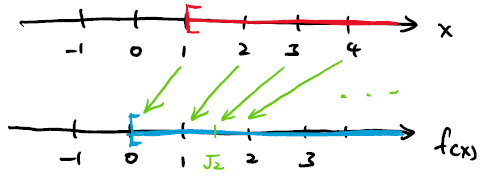
\includegraphics[width=0.4\textwidth]{sqrt_x-1}
\end{center}


%%%%%%%%%%%%%%
\subsection{Multivariable Scalar Function}

\begin{itemize}
    \item Domain = A set of tuples of number, like $x = (1,2,3)$
    \item Image = A set of single number, like $f(x) = 5$
\end{itemize}

For example,
\aleq{
    f(x,y) = \sqrt{1-xy} \qquad \Rightarrow \qquad 
    \bcase{
        \text{\red{Domain} } &= \text{Any pair of values }x,y\text{ where } xy\leq 1 \\
        \text{\blue{Image} } &= \text{ Any real number }\geq 0
    }
}

\begin{center}
    \begin{minipage}{0.15\textwidth}
        \red{
            $(x,y)$ can be\\
            any point in\\
            this region
        }
    \end{minipage}
    %
    \begin{minipage}{0.3\textwidth}
        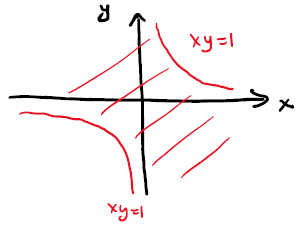
\includegraphics[height=9em]{sqrt_1-xy_D}
    \end{minipage}
    %
    \green{$\xrightarrow{\hspace{0.2\textwidth}}$}
    %
    \begin{minipage}{0.22\textwidth}
        \centering
        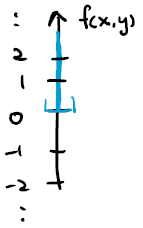
\includegraphics[height=9em]{sqrt_1-xy_I}
    \end{minipage}
\end{center}

\ul{Example in Physics:}
\begin{itemize}
    \item Gravitational potential energy
    \aleq{
        U(x,y,z) = -\frac{GMm}{r} = -\frac{GMm}{\sqrt{x^2+y^2+z^2}}
    }
\end{itemize}

\begin{minipage}[t]{0.5\textwidth}
    \begin{itemize}
        \item Density distribution in object $\rho(x,y,z)$
    \end{itemize}
\end{minipage}
\begin{minipage}[t]{0.48\textwidth}
    \begin{figure}[t]
        \strut\vspace*{-\baselineskip}\newline
        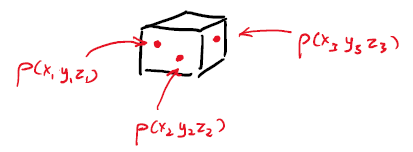
\includegraphics[width=0.75\textwidth]{density}
    \end{figure}
    
\end{minipage}

%%%%%%%%%%%%%%
\subsection{Single Variable Vector Function}

\begin{itemize}
    \item Domain = A set of single number
    \item Image = A set of tuple of numbers
\end{itemize}

For example,
\aleq{
    \vvec{r}(t) = (x(t), y(t)) = (t^2, 3t^3) \qquad \Rightarrow \qquad 
    \bcase{
        \text{\red{Domain} } &= \text{Any real number } t \\
        \text{\blue{Image} } &= (x,y) \text{ pairs restricting on } x=\qty(\frac{y}{3})^{\frac{2}{3}}
    }
}

\begin{center}
    \begin{minipage}{0.15\textwidth}
        \red{
            $t$ can be any\\
            real number
        }
    \end{minipage}
    %
    \begin{minipage}{0.15\textwidth}
        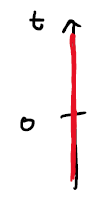
\includegraphics[height=9em]{t2_3t3_D}
    \end{minipage}
    %
    \green{$\xrightarrow{\hspace{0.15\textwidth}}$}
    %
    \begin{minipage}{0.3\textwidth}
        \centering
        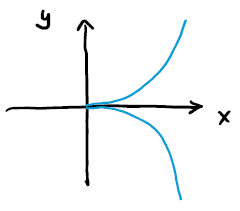
\includegraphics[height=9em]{t2_3t3_I}
    \end{minipage}
    %
    \begin{minipage}{0.15\textwidth}
        \blue{
            \aleq{
                x=t^2 &\text{ and } y=3t^3 \\
                \Rightarrow x &= \qty(\dfrac{y}{3})^{\frac{3}{2}}
            }
        }
    \end{minipage}
\end{center}

\ul{Example in Physics:}
\begin{itemize}
    \item Displacement, velocity, acceleration
    \aleq{
        \bcase{
            \vvec{s}(t) &= (x(t), y(t), z(t)) \\
            \vvec{v}(t) &= (v_x(t), v_y(t), v_z(t)) \\
            \vvec{a}(t) &= (a_x(t), a_y(t), a_z(t))
        }
    }
\end{itemize}

%%%%%%%%%%%%%%
\subsection{Multivariable Vector Function}

\begin{itemize}
    \item Domain = A set of tuple of numbers
    \item Image = A set of tuple of numbers
\end{itemize}

For example,
\aleq{
    \vvec{r}(u,v) = (r_1(u,v), r_2(u,v)) = (u^2+v^2, u-1-v^2) \qquad \Rightarrow \qquad 
    \bcase{
        \text{\red{Domain} } &= \text{The whole u-v plane} \\
        \text{\blue{Image} } &= \text{ Region depicted below}
    }
}

\begin{center}
    \begin{minipage}{0.3\textwidth}
        \centering
        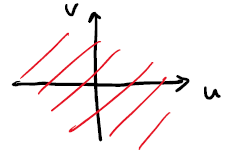
\includegraphics[height=7em]{ruv_D}
    \end{minipage}
    %
    \green{$\xrightarrow{\hspace{0.2\textwidth}}$}
    %
    \begin{minipage}{0.3\textwidth}
        \centering
        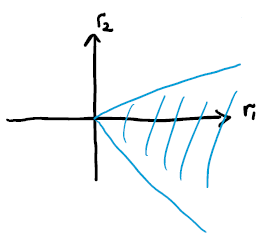
\includegraphics[height=9em]{ruv_I}
    \end{minipage}
    %
    \begin{minipage}{0.15\textwidth}
        \blue{
            Any point in\\
            this region,\\
            estimated on\\
            computer
        }
    \end{minipage}
\end{center}

\ul{Example in Physics:}
\begin{itemize}
    \item Gravitational force
    \aleq{
        \vvec{F}(\vvec{r}) &= \vvec{F}(x,y,z)\\
        &= -\frac{GMm}{|\vvec{r}|^2}\cdot \red{\qty(\frac{\vvec{r}}{|\vvec{r}|})} \tkm{runit}\\
        &= -\frac{GMm}{x^2+y^2+z^2} \cdot \qty(
        \frac{\green{x}\blue{\hhat{x}} + \green{y}\blue{\hhat{y}} + \green{z}\blue{\hhat{z}}
        }{\sqrt{x^2+y^2+z^2}}) \tkm{sep_component}\\
        &= \qty[\frac{-GMm\green{x}}{(x^2+y^2+z^2)^{\frac{3}{2}}}]\blue{\hhat{x}}
        + \qty[\frac{-GMm\green{y}}{(x^2+y^2+z^2)^{\frac{3}{2}}}]\blue{\hhat{y}}
        + \qty[\frac{-GMm\green{z}}{(x^2+y^2+z^2)^{\frac{3}{2}}}]\blue{\hhat{z}}
    }
    \addArrow[red]{runit}{(5ex, 0)}{Unit vector of $\vvec{r}$}{(2ex,0)}{(8ex,0)}
    \addArrow[blue]{sep_component}{(5ex, 0)}{Separate into components of $\hhat{x}/\hhat{y}/\hhat{z}$}{(2ex,0)}{(18ex,0)}
\end{itemize}

%%%%%%%%%%%%%%
\subsection{Function Composition for multivariable functions}

For single variable scalar function, you should be familiar with the what function composition is. 
For example, if $f(x) = \sin{x}, g(x) = e^{x}$, we can have these compositions:

\aleq{
    f(f(x)) = \sin{(\sin{x})} \quad,\quad 
    f(g(x)) = \sin{(e^x)} \quad, \quad 
    g(f(x)) = e^{\sin{x}} \quad, \quad
    g(g(x)) = e^{e^x}
}

Note that function composition is the key in chain rule. 

\aleq{
    \dvv{x}f(g(x)) = \dvv{f(g(x))}{g(x)}\cdot \dvv{g(x)}{x}
}

However for multivariable functions, we can construct function composition only if 
the number of output matches the next function's number of input. For example, let's have
\aleq{
    \bcase{
        f(p,q) &= \sqrt{p+q} \qquad \blue{\text{2 inputs, 1 output. Denote as }(2 \xrightarrow{f} 1)} \\
        \vvec{g}(t) &= (t-1, t^2) \qquad \blue{\text{1 input, 2 outputs. Denote as }(1 \xrightarrow{g} 2)} \\
        \vvec{h}(u,v) &= (u^2+v, u-v) \qquad \blue{\text{2 inputs, 2 outputs. Denote as }(2 \xrightarrow{h} 2)}
    }
}

We can have the following composition:
\aleq{
    f(\vvec{g}(t)) &= \sqrt{(t-1) + (t^2)} \qquad \blue{(1 \xrightarrow{g} 2 \xrightarrow{f} 1)} \\
    f(\vvec{h}(u,v)) &= \sqrt{(u^2+v) + (u-v)} \qquad \blue{(2 \xrightarrow{h} 2 \xrightarrow{f} 1)} \\
    \vvec{g}(f(p,q)) &= (\sqrt{p+q}-1, p+q) \qquad \blue{(2 \xrightarrow{f} 1 \xrightarrow{g} 2)} \\
    \vvec{h}(\vvec{g}(t)) &= ((t-1)^2+(t^2), (t-1)-(t^2)) \qquad \blue{(1 \xrightarrow{g} 2 \xrightarrow{h} 2)} \\
    \vvec{h}(\vvec{h}(t)) &= ((u^2+v)^2+(u-v), (u^2+v)-(u-v)) \qquad \blue{(2 \xrightarrow{h} 2 \xrightarrow{h} 2)}
}

But these are NOT allowed:
\aleq{
    g(h(u,v)) \quad &\colon \quad \blue{(2 \xrightarrow{h} 2 \ \red{\Rightarrow}\ 1 \xrightarrow{g} 2)} \\
    h(f(p,q)) \quad &\colon \quad \blue{(2 \xrightarrow{f} 1 \ \red{\Rightarrow}\ 2 \xrightarrow{h} 2)}
}

\linesep
% Section %%%%%%%%%%%%%%%%%%%%%%%%%%%%%%%%%%%%%%%%%%%%%%%%%%%%
\section{Limits on Multivariable Scalar Function}

In single variable functions, $\lim_{x\to a} f(x) = L$ means 
when the input $x$ is "close enough" to a value $a$, output of $f(x)$ must be "close" to some $L$.
This idea can be extended to multivariable function, i.e.
\aleq{
    \lim_{(x_1,x_2,...,x_n)\to(a_1,a_2,...,a_n)} f(x_1, x_2,...,x_n) = L
}

The idea requires all the inputs $x_1, x_2, ...$ to be "close enough" to some corresponding values $a_1, a_2,...$,
only after then the output of $f(...)$ will be "close" enough to some $L$. 
We can visually compare it with single variable function as follow:\\

\begin{center}
    \begin{minipage}{0.45\textwidth}
        \centering
        \ul{Single Variable Function}
        \\[1em]
        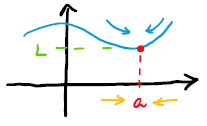
\includegraphics[height=6em]{limit_sing}
        \\
        $x$ can approach $a$ \\
        from either left or right
    \end{minipage}
    %
    \begin{minipage}{0.45\textwidth}
        \centering
        \ul{Multivariable Function}
        \\[1em]
        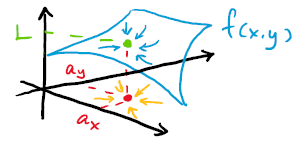
\includegraphics[height=6em]{limit_mul}
        \\
        $x$ can approach $a$ \\
        from every direction
    \end{minipage}
\end{center}

Therefore, the "existance" of limit in multivariable functions has a much stricter requirement.
\begin{itemize}
    \item Single variable function: 
    \begin{itemize}
        \item Input $x$ must approach the point $a$ from either left ($x^-$) or right ($x^+$).
        \item "Existance" of limit only require showing both left/right limits approach to the same output $L$.
    \end{itemize}
    
    \item Multivariable function, (e.g. functions with 2 inputs):
    \begin{itemize}
        \item Inputs $(x_1, x_2)$ can approach the point $(a_1, a_2)$ along any trajectories on the plane. 
        \item "Existance" of limit require showing that along ALL trajectories.
    \end{itemize}
\end{itemize}


 Proving a limit exist rigorously is a lot harder in multivariable function.
 But in physics, we almost never need to deal with any strange functions that has limit only along certain trajectories.
 \red{We may assume that every function we encounter is well-behaved, 
 and then calculation can be done like in single variable functions.} E.g.

\aleq{
    \lim_{(x,y)\to \qty(\frac{\pi}{2},\frac{\pi}{2})} \sin{x}\cos{y} = \sin\qty(\frac{\pi}{2})\cos\qty(\frac{\pi}{2})
}
 





\linesep
% Section %%%%%%%%%%%%%%%%%%%%%%%%%%%%%%%%%%%%%%%%%%%%%%%%%%%%
\section{Partial Differentiation}

\begin{itemize}
    \item Notation: $\pdvv{x}, \pdvv{y}, ...$
    \item Usually pronouced as "partial x", "partial y", etc.
\end{itemize}

Comparing with ordinary differentiation to single variable function, 
the notation difference is to emphasize that the \bf{differentiation is only about 1 of the inputs}. 

%%%%%%%%%%%%%%
\subsection{Definition \& Geometrical Interpretation}

The limit definition of partial differentiation of $f(x_1, x_2,..., x_n)$ at $(a_1, a_2,...,a_n)$ in the i$^{th}$ input (\red{$x_i$}) 's direction is defined as:
\aleq{
    &\pdvv{\red{x_i}}f(x_1, x_2,...,\red{x_i},...,x_n) \\
    = &\lim_{\red{\Delta x_i \to 0}} \qty[\frac{f(x_1,x_2,...,\red{x_i+\Delta x_i},...,x_n) - f(x_1, x_2,...,\red{x_i},...,x_n)}{\red{\Delta x_i}}]
}

Note that \red{the limit only acts on the i$^{th}$ input.} Other inputs remains untouched.\\

Therefore in calculation, when doing partial differentiation over $x_i$,
only $x_i$ is differentiated (the same way we do in single variable differentiation), while the other $x$ are treated as constants.\\

E.g. $f(x,y,z) = x^2y\sin{z}$
\aleq{
    \pdvv{f}{\red{x}} &= \red{2x}\cdot y\sin{z} &\qty(\dvv{x}x^2 = 2x, \text{don't touch }y,z)\\
    \pdvv{f}{\red{y}} &= x^2 \cdot \red{1} \cdot \sin{z} &\qty(\dvv{y}y = 1, \text{don't touch }x,z)\\
    \pdvv{f}{\red{z}} &= x^2y\cdot \red{\cos{z}} &\qty(\dvv{z}\sin{z} \cos{z}, \text{don't touch }x,y)
}

The visualization to partial differentiation is straightforward. 
Take a 2-inputs function $f(x,y)$ as example, we can demonstrate by the following illustrations:

\begin{center}
    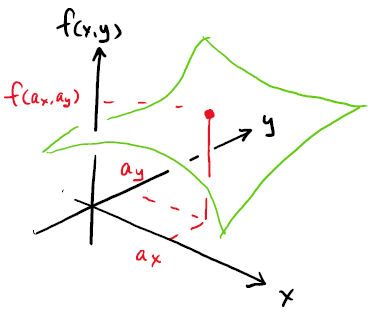
\includegraphics[height=12em]{pdv}
    \\[1em]
    \begin{minipage}{0.48\textwidth}
        \centering
        \yellow{\ul{Make a slice at $y=a_y$}}\\
        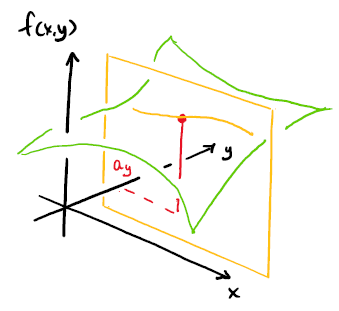
\includegraphics[height=12em]{pdx}
        \\
        \yellow{\Large $\Downarrow$}
        \\
        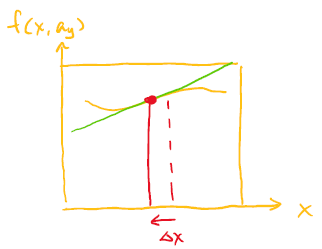
\includegraphics[height=12em]{pdx_sec}
        \\
        $\pdvv{x}$ = On the plane of constant $y$, \\
        \hspace{6ex} find slope along $x$ direction.
    \end{minipage}
    %
    \hfill\vline\hfill
    %
    \begin{minipage}{0.48\textwidth}
        \centering
        \blue{\ul{Make a slice at $x=a_x$}}\\
        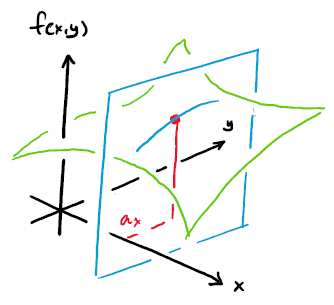
\includegraphics[height=12em]{pdy}
        \\
        \blue{\Large $\Downarrow$}
        \\
        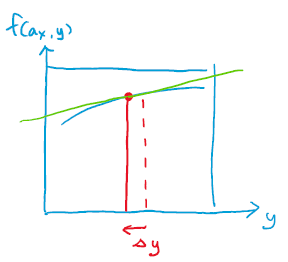
\includegraphics[height=12em]{pdy_sec}
        \\
        $\pdvv{y}$ = On the plane of constant $x$, \\
        \hspace{6ex} find slope along $y$ direction.
    \end{minipage}
\end{center}


\newpage
We can conclude:
\begin{center}
    \begin{minipage}{0.75\textwidth}
        \begin{framed}
            \centering
            $\pdvv{x_i}$ = Find slope / rate of change of function with respect to $x_i$
        \end{framed}
    \end{minipage}
\end{center}

    


%%%%%%%%%%%%%%
\subsection{Evaluating Partial Differentiation}

\red{Calculation rules for partial differentation are all the same as in single variable functions except chain rule.} 
Due to how function composition works in multivariable calculus, 
the multivariable version is the \bf{sum of chain rule with respect to each of the input.}

\aleq{
    \pdvv{x_i}f(\vvec{g}(x_1,x_2,...,x_n)) &= \sum_j \pdvv{g_j}f(\vvec{g})\pdvv{g_j}{x_i} \\
    &= \pdvv{g_1}f(\vvec{g})\pdvv{x_i}g_1(x_1,x_2,...,x_n) + \pdvv{g_2}f(\vvec{g})\pdvv{x_i}g_2(x_1,x_2,...,x_n) + ...
}

\it{As for now you do not need to remember this formula. We will be able to write it in a more compact (and easier to remember) form after learning matrix.}\\

As an example of calculation, suppose we start with two functions without knowing their exact expression: 
\aleq{
    f(p,q) & &\qquad \blue{(2 \xrightarrow{f} 1)} \\
    \vvec{h}(u,v) &= (h_1(u,v), h_2(u,v)) = (h_1,h_2)  &\qquad \blue{(2 \xrightarrow{h} 2)}
}
And construct the following composition:
\aleq{
    f(\vec{h}(u,v)) &= f((h_1, h_2))= f((h_1(u,v), h_2(u,v))) &\qquad \blue{(2 \xrightarrow{h} 2 \xrightarrow{h} 1)}
}

Because $f(\vec{h}(u,v))$ takes 2 inputs $u,v$, there must be 2 partial differentiations (one for $u$ and one for $v$).
With chain rule, the partial differentiations write as \\

With respect to $u$:
\aleq{
    \pdvv{u}f(\vvec{h}(u,v)) &= \pdvv{\tkn{uu}{\cul[red]{\cul[blue]{u}}}} f
        (\tkn{h11}{\cul[red]{h_1}}, \tkn{h12}{\cul[blue]{h_2}}) \\[2.5em]
        %
    &= \cub[red]{{\qty(\pdvv{\cbox[red]{h_1}}f(\cbox[red]{h_1},h_2) \cdot \cbox[red]{\pdvv{u}h_1})}}{\text{Chain rule over }h_1 \text{ only}} 
        + \cub[blue]{\qty(\pdvv{\cbox[blue]{h_2}}f(h_1,\cbox[blue]{h_2})\cbox[blue]{\pdvv{u}h_2})}{\text{Chain rule over } h_2 \text{ only}}
}
\addUnderArrow[red]{uu}{h11}{$u$ on $h_1$ }{-2ex}{(0,0)}{(0,-0.5ex)}
\addAboveArrow[blue]{uu}{h12}{$u$ on $h_2$}{5ex}{(0.5ex,-0.5ex)}

With respect to $v$:
\aleq{
    \pdvv{v}f(\vvec{h}(u,v)) &= \pdvv{\tkn{vv}{\cul[red]{\cul[blue]{v}}}} f
        (\tkn{h21}{\cul[red]{h_1}}, \tkn{h22}{\cul[blue]{h_2}}) \\[2.5em]
        %
    &= \cub[red]{{\qty(\pdvv{\cbox[red]{h_1}}f(\cbox[red]{h_1},h_2) \cdot \cbox[red]{\pdvv{v}h_1})}}{\text{Chain rule over }h_1 \text{ only}} 
        + \cub[blue]{\qty(\pdvv{\cbox[blue]{h_2}}f(h_1,\cbox[blue]{h_2})\cbox[blue]{\pdvv{v}h_2})}{\text{Chain rule over } h_2 \text{ only}}
}
\addUnderArrow[red]{vv}{h21}{$v$ on $h_1$ }{-2ex}{(0,0)}{(0,-0.5ex)}
\addAboveArrow[blue]{vv}{h22}{$v$ on $h_2$}{5ex}{(0.5ex,-0.5ex)}

We may do straightforward substitution, if the functions' expressions are given. Let's say,   
\aleq{
    f(p,q) &= \sqrt{p+q} \qquad \text{and}\qquad \vvec{h}(u,v) = (u^2+v, u-v) = (h_1, h_2)
}

Then 
\aleq{
    \pdvv{u}f(\vvec{h}(u,v)) 
    &= \cul[red]{\qty(\pdvv{h_1}f(h_1, h_2)\pdvv{u}h_1)} + \cul[blue]{\qty(\pdvv{h_2}f(h_1, h_2)\pdvv{u}h_2)} \\[1em]
    &= \cul[red]{\qty(\pdvv{h_1}\sqrt{h_1+h_2}\eval_{\substack{h_1=u^2+v \\ h_2=u-v}} \cdot \pdvv{u}(u^2+v))}  
        + \cul[blue]{\qty(\pdvv{h_2}\sqrt{h_1+h_2} \eval_{\substack{h_1=u^2+v \\ h_2=u-v}}\cdot \pdvv{u}(u-v))}  \\[1em]
    &= \cul[red]{\qty(\inv{2\sqrt{h_1+h_2}}\eval_{\substack{h_1=u^2+v \\ h_2=u-v}}\cdot 2u)}
         + \cul[blue]{\qty(\inv{2\sqrt{h_1+h_2}}\eval_{\substack{h_1=u^2+v \\ h_2=u-v}}\cdot (1))} \\[1em]
    &= \frac{2u}{2\sqrt{u^2+u}} + \frac{1}{2\sqrt{u^2+u}} \\[1em]
    &= \frac{2u+1}{2\sqrt{u^2+u}}\\[1em]
    %
    \pdvv{v}f(\vvec{h}(u,v)) 
    &= \cul[red]{\qty(\pdvv{h_1}f(h_1, h_2)\pdvv{v}h_1)} + \cul[blue]{\qty(\pdvv{h_2}f(h_1, h_2)\pdvv{v}h_2)} \\[1em]
    &= \cul[red]{\qty(\pdvv{h_1}\sqrt{h_1+h_2}\eval_{\substack{h_1=u^2+v \\ h_2=u-v}} \cdot \pdvv{v}(u^2+v))}  
        + \cul[blue]{\qty(\pdvv{h_2}\sqrt{h_1+h_2} \eval_{\substack{h_1=u^2+v \\ h_2=u-v}}\cdot \pdvv{v}(u-v))}  \\[1em]
    &= \cul[red]{\qty(\inv{2\sqrt{h_1+h_2}}\eval_{\substack{h_1=u^2+v \\ h_2=u-v}}\cdot (1))}
         + \cul[blue]{\qty(\inv{2\sqrt{h_1+h_2}}\eval_{\substack{h_1=u^2+v \\ h_2=u-v}}\cdot (-1))} \\[1em]
    &= \frac{1}{2\sqrt{u^2+u}} + \frac{-1}{2\sqrt{u^2+u}} \\[1em]
    &= 0
}

We can also compute the composition directly for result checking:
\aleq{
    f(\vvec{h}(u,v)) = \sqrt{u^2+v + u-v} = \sqrt{u^2+u}
}
\aleq{
    \Rightarrow\quad \pdvv{f}{u} = \frac{2u+1}{2\sqrt{u^2+u}} \qquad \text{and} \qquad \pdvv{f}{v} = 0
}

\begin{exercise}
    Given the functions and their composition: 
    \aleq{
        \begin{cases}
            f(p,q)=\sqrt{p+q} \\ \vvec{g}(t) = (t-1,t^2)
        \end{cases}
        \qquad \Rightarrow \qquad
        f(\vvec{g}(t)) = \sqrt{t^2+t-1}
    }
    Compute the derivative $\dvv{t}f(\vvec{g}(t))$, by
    \begin{enumerate}
        \item directly differentiating against $t$
        \item first differentiate via chain rule over $(p,q)$
    \end{enumerate}
    (You should get equal results.)
\end{exercise}



\linesep
% Section %%%%%%%%%%%%%%%%%%%%%%%%%%%%%%%%%%%%%%%%%%%%%%%%%%%%
\section{Multiple Integral}

The limit definition of multiple integral can be written as

\aleq{
    &\idotsint_\red{\qty(\substack{\text{Some}\\\text{region}})}
    f(x_1, x_2,...,x_n) \dd{x_1}\dd{x_2}...\dd{x_n} \\
    = & 
    \lim_{\Delta x_1, \Delta x_2,...,\Delta x_n \to 0} \sum_{\red{\substack{\text{all divisions}\\\text{in the region}}}}
    f(\xi_1, \xi_2, ..., \xi_n) \Delta x_1 \Delta x_2...\Delta x_n 
}

Recall that we have introduced 2 geometrical interpretations of integration.
Here we can demonstrate them on the two most frequently used multiple integral.

%%%%%%%%%%%%%%
\subsection{Double Integral}

For functions with 2 inputs.\\

\ul{Interpretation 1: Volume under surface, bounded by base area}

\aleq{
    \iint_{\red{\substack{\text{Some}\\\text{Area}}}} f(x,y) \dd{x}\dd{y} 
    = \lim_{\Delta x, \Delta y \to 0} \sum_{\red{\substack{\text{All divisions}\\\text{in the area}}}} 
    \tkn{pillar_h}{\cul[blue]{f(\xi_x, \xi_y)}} \tkn{pillar_a}{\cul[yellow]{\Delta x\Delta y}}
}\\
\addArrow[blue]{pillar_h}{(0,-4.5ex)}{Pillar's height}{(0,-2ex)}
\addArrow[yellow]{pillar_a}{(4ex,-4ex)}{Pillar's base area}{(0,-2ex)}{(7ex,0)}

\begin{center}
    \begin{minipage}{0.6\textwidth}
        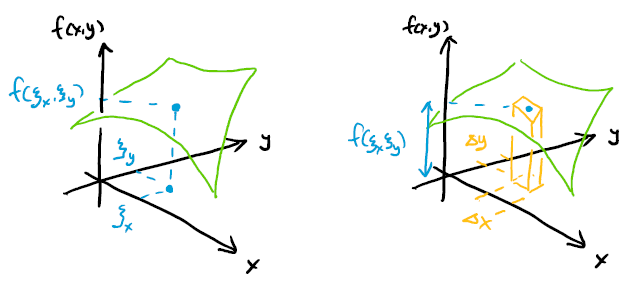
\includegraphics[width=\textwidth]{iint_pillar}
    \end{minipage}
    %
    \begin{minipage}{0.3\textwidth}
        \centering
        \yellow{One pillar for every point}
    \end{minipage}
\end{center}

\begin{center}
    \begin{minipage}{0.4\textwidth}
        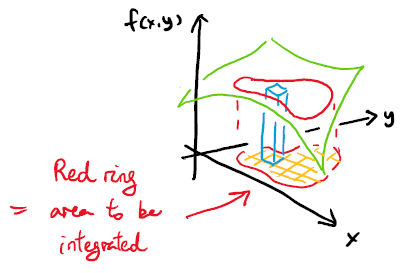
\includegraphics[width=\textwidth]{iint_reg}
    \end{minipage}
    %
    \hspace{0.05\textwidth}
    %
    \begin{minipage}{0.4\textwidth}
        \centering
        \begin{framed}
            Double integral \\
            = Sum the volumes of all pillars\\
            within the red ring (region)
        \end{framed}
    \end{minipage}
\end{center}



\ul{Interpretation 2: Weighted sum over an area}

\aleq{
    \iint_{\red{\substack{\text{Some}\\\text{Area}}}} f(x,y) \dd{x}\dd{y} 
    = \lim_{\Delta x, \Delta y \to 0} \sum_{\red{\substack{\text{All divisions}\\\text{in the area}}}} 
    \tkn{weight2}{\cul[blue]{f(\xi_x, \xi_y)}} \tkn{area2}{\cul[yellow]{\Delta x\Delta y}}
}\\
\addArrow[blue]{weight2}{(0,-6ex)}{Weight for the\\grid at $(\xi_x,\xi_y)$}{(0,-2ex)}{(0,-1ex)}
\addArrow[yellow]{area2}{(4ex,-4ex)}{Area of each grid}{(0,-2ex)}{(7ex,0)}


\begin{center}
    \begin{minipage}{0.4\textwidth}
        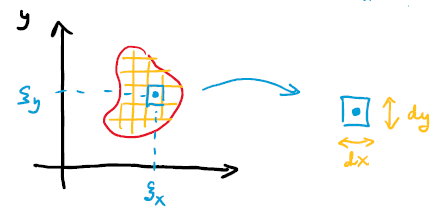
\includegraphics[width=\textwidth]{iint_weight}
    \end{minipage}
    %
    \hspace{0.05\textwidth}
    %
    \begin{minipage}{0.5\textwidth}
        \centering
        \begin{framed}
            Double integral \\
            = For each grid of weight $f(\xi_x,\xi_y)$,\\
            Sum all grids within the red ring (region)
        \end{framed}
    \end{minipage}
\end{center}

For a physics example, the \it{area mass density distribution} $\sigma(x,y)$ may depends on position coordinate $(x,y)$.
\begin{itemize}
    \item Each small grid has an area $(\dd{x} \dd{y})$
    \item At position $(\xi_x, \xi_y)$, the grid has a density $\sigma(x,y)$
\end{itemize}

Thus, 
\aleq{
    \text{Total mass} &= \text{Sum of mass of all small grids}\\[1em]
    &= \sum_{\substack{\text{all small grids}\\\text{in the area}}} \qty(\substack{\text{density}\\\text{of each grid}})\qty(\substack{\text{area}\\\text{of each grid}}) \\[1em]
    &= \sum_{\substack{\text{all small grids}\\\text{in the area}}} \sigma(x,y) \cdot (\Delta x \Delta y) \\[1em]
    &\approx \iint_{\text{the area}} \sigma(x,y) \dd{x}\dd{y}
}


%%%%%%%%%%%%%%
\subsection{Triple Integral}

\ul{Interpretation 1: ??? under volume}

\begin{center}
(Sorry, we live in a 3D space. No idea how to draw 4D objects.)\\
\end{center}


\ul{Interpretation 2: Weighted sum over a volume}

\aleq{
    \iiint_{\red{\substack{\text{Some}\\\text{Volume}}}} f(x,y,z) \dd{x}\dd{y}\dd{z}
    = \lim_{\Delta x, \Delta y, \Delta z \to 0} \sum_{\red{\substack{\text{All divisions}\\\text{in the volume}}}} 
    \tkn{weight3}{\cul[blue]{f(\xi_x, \xi_y, \xi_z)}} \tkn{vol3}{\cul[yellow]{\Delta x\Delta y \Delta z}}
}
\addArrow[blue]{weight3}{(0,-6ex)}{Weight for the\\cube at $(\xi_x,\xi_y,\xi_z)$}{(0,-2ex)}{(0,-1ex)}
\addArrow[yellow]{vol3}{(4ex,-4ex)}{Volume of each cube}{(0,-2ex)}{(7ex,0)}

\begin{center}
    \begin{minipage}{0.4\textwidth}
        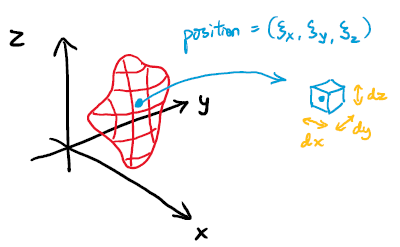
\includegraphics[width=\textwidth]{iiint_weight}
    \end{minipage}
    %
    \hspace{0.05\textwidth}
    %
    \begin{minipage}{0.5\textwidth}
        \centering
        \begin{framed}
            Triple integral \\
            = For each cube of weight $f(\xi_x,\xi_y, \xi_z)$,\\
            Sum all cubes within the red region
        \end{framed}
    \end{minipage}
\end{center}

Similar to double integral, if $\rho(x,y,z)$ is the \it{volume mass density distribution}, 
then, 
\aleq{
    \text{Total mass} &= \text{Sum of mass of all small cubes}\\[1em]
    &= \sum_{\substack{\text{all small cubes}\\\text{in the volume}}} \qty(\substack{\text{density}\\\text{of each cube}})\qty(\substack{\text{volume}\\\text{of each cube}}) \\[1em]
    &= \sum_{\substack{\text{all small cubes}\\\text{in the volume}}} \rho(x,y,z) \cdot (\Delta x \Delta y \Delta z) \\[1em]
    &\approx \iiint_{\text{the volume}} \rho(x,y,z) \dd{x}\dd{y}\dd{z}
}


%%%%%%%%%%%%%%
\subsection{Evaluating Multiple Integral}

The difficulty in calculation mostly comes from determining the region to be integrated.
Here are the main steps in your calculation:

\begin{enumerate}
    \item Decide the integration order, i.e. how to divide a region.
    \begin{itemize}
        
        \item The integration order decide the expression. Follow the expression to integrate "from inside to outside".
        \aleq{
            \iiint f(x,y,z) \dd{x}\dd{y}\dd{z} = \yellow{\tkn{out}{\int}\qty(\blue{\tkn{mid}{\int}\qty(\tkn{in}{\red{\int f(x,y,z)\dd{x}}})\dd{y}})\dd{z}}
        }\\
        \addArrow[red]{in}{(4ex,-3ex)}{inner = \nth{1}}{(0,-2ex)}{(2ex,0)}
        \addArrow[blue]{mid}{(0,-3ex)}{middle = \nth{2}}{(0,-2ex)}
        \addArrow[yellow]{out}{(-8ex,-3ex)}{outer = \nth{3}}{(0,-2ex)}{(-4ex,0)}

        \item Calculation is exactly how you do single variable integration, but do it multiple times. 
        \item While integrating one variable, treat the others as constants.
    \end{itemize}

    \item Derive the corresponding upper/lower bounds
    \begin{itemize}
        \item It would be easier if you can draw out the region.
        \item Note that if you switch the integration order, the bounds must change.
    \end{itemize}

\end{enumerate}


\begin{example}
    Integrate $f(x,y) = x^2y-xy^3$ over the region bounded by 
    $\begin{cases}x&=1\\x&=4\end{cases}$ and $\begin{cases}y&=2\\y&=3\end{cases}$

    \begin{center}
        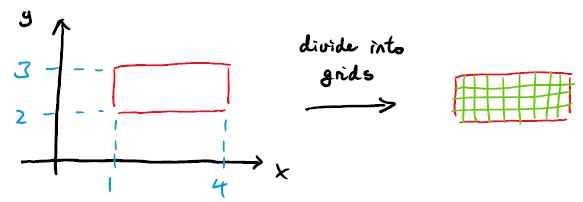
\includegraphics[width=0.6\textwidth]{iint_eg}
    \end{center}

    \ul{Integration order 1:} First $x$, then $y$.
    \begin{enumerate}
        \item Integrate $x$ = Sum all grid with the same $y$ coordinate to form horizontal strips.
        
        \begin{center}
            \begin{minipage}{0.55\textwidth}
                \centering
                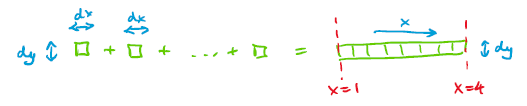
\includegraphics[width=0.95\textwidth]{iint_eg_x}
            \end{minipage}
            %
            $\displaystyle \Rightarrow \quad  \int_{x=1}^{x=4}f(x,y)\dd{x}$
        \end{center}

        
        \item Integrate $y$ = Sum all horizontal strips to from the integration region.
        
        \begin{center}
            \begin{minipage}{0.55\textwidth}
                \centering
                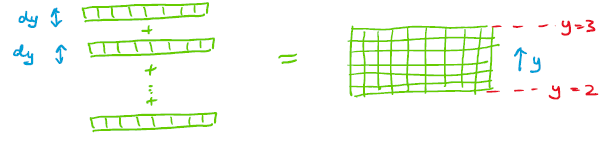
\includegraphics[width=0.95\textwidth]{iint_eg_xy}
            \end{minipage}
            %
            $\displaystyle \Rightarrow \quad  \int_{y=2}^{y=3}\qty[\int_{x=1}^{y=4}f(x,y)\dd{x}]\dd{y}$
        \end{center}

        \item In the calculation, follow the expression's order: Integrate $x$ first, then $y$. 
        Note that before integrating $y$, you need to clear all $x$ by substituting the given upper/lower bounds.
        \aleq{
            &\int_{y=2}^{y=3}\red{\qty[\int_{x=1}^{y=4}x^2y-xy^3\dd{x}]}\dd{y}\\[1em]
            = &\int_{y=2}^{y=3}\red{\qty[\frac{x^3}{3}y - \frac{x^2}{2}y^3]\eval_{x=1}^{x=4}}\dd{y}\\[1em]
            = &\int_{y=2}^{y=3} \cub[red]{\qty(\frac{64}{3}y-\frac{16}{2}y^3)}{\text{Subst. }x=4} - \cub[red]{\qty(\frac{1}{3}y - \half y^3)}{\text{Subst. }x=1} \dd{y} \\[1em]
            = &\int_{y=2}^{y=3} 21y - \frac{15}{2}y^3 \dd{y} \\[1em]
            = &\qty[\frac{21}{2}y^2-\frac{15}{8}y^4]\eval_{y=2}^{y=3} \\[1em]
            = &\frac{-555}{8}
        }
    \end{enumerate}

    \ul{Integration order 2:} First $y$, then $x$.
    \begin{enumerate}
        \item Integrate $y$ = Sum all grid with the same $x$ coordinate to form vertical strips.
        
        \begin{center}
            \begin{minipage}{0.35\textwidth}
                \centering
                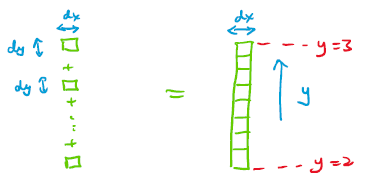
\includegraphics[width=0.95\textwidth]{iint_eg_y}
            \end{minipage}
            %
            $\displaystyle \Rightarrow \quad  \int_{y=3}^{y=2}f(x,y)\dd{y}$
        \end{center}

        
        \item Integrate $y$ = Sum all horizontal strips to from the integration region.
        
        \begin{center}
            \begin{minipage}{0.55\textwidth}
                \centering
                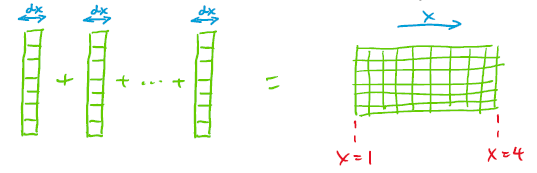
\includegraphics[width=0.95\textwidth]{iint_eg_yx}
            \end{minipage}
            %
            $\displaystyle \Rightarrow \quad  \int_{x=1}^{x=4}\qty[\int_{y=2}^{y=3}f(x,y)\dd{y}]\dd{x}$
        \end{center}

        \newpage
        \item In the calculation, follow the expression's order: Integrate $y$ first, then $x$. 
        Note that before integrating $x$, you need to clear all $y$ by substituting the given upper/lower bounds.
        \aleq{
            &\int_{x=1}^{x=4}\red{\qty[\int_{y=2}^{y=3}x^2y-xy^3\dd{y}]}\dd{x}\\[1em]
            = &\int_{x=1}^{x=4}\red{\qty[\half x^2y^2 - \inv{4}xy^4]\eval_{y=2}^{y=3}}\dd{x}\\[1em]
            = &\int_{x=1}^{x=4} \cub[red]{\qty(\frac{9}{2}x^2 - \frac{81}{4}x)}{\text{Subst. }y=3} - \cub[red]{\qty(2x^2-4x)}{\text{Subst. }y=2} \dd{x} \\[1em]
            = &\int_{x=1}^{x=4} \frac{5}{2}x^2 - \frac{65}{4}x \dd{x} \\[1em]
            = &\qty[\frac{5}{6}x^3-\frac{65}{8}x^2]\eval_{x=1}^{x=4} \\[1em]
            = &\frac{-555}{8}
        }
    \end{enumerate}

\end{example}

However, if the boundaries of the region is ugly, 
some integration order make your life easier than the others.

\begin{example}

    Consider integration over the below region (with an arbituary $f(x,y)$):

    \begin{center}
        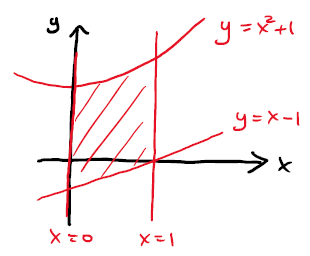
\includegraphics[width=0.25\textwidth]{iint_eg2}
    \end{center}

    \ul{Integration order 1:} First $y$, then $x$.

    \begin{center}
        \begin{minipage}{0.4\textwidth}
            \centering
            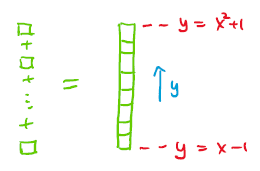
\includegraphics[width=0.55\textwidth]{iint_eg2_y}
        \end{minipage}
        %
        then
        %
        \begin{minipage}{0.5\textwidth}
            \centering
            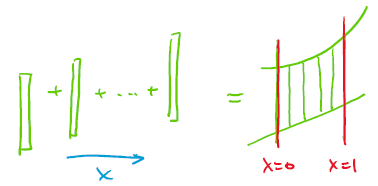
\includegraphics[width=0.7\textwidth]{iint_eg2_yx}
        \end{minipage}
    \end{center}

    This approach is easy because all vertical strips have the same bounds:
    \begin{itemize}
        \item Upper bound: The curve $y=x^2+1$
        \item Lower bound: The curve $y=x-1$
    \end{itemize}

    We can write the integral expression as a single term.
    \aleq{
        \int_{x=0}^{x=1}\int_{y=x-1}^{y=x^2+1} f(x,y) \dd{y}\dd{x}
    }

    \ul{Integration order 2:} First $x$, then $y$.\\

    Note that the bounds of horizontal strips are different for different $y$:

    \begin{center}
        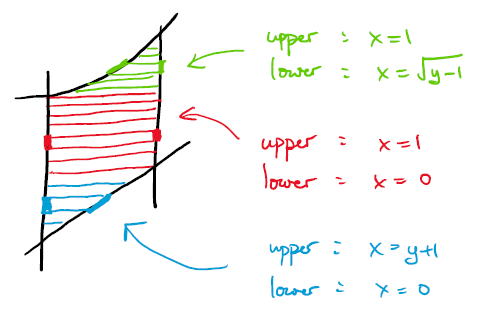
\includegraphics[width=0.45\textwidth]{iint_eg2_x}
    \end{center}

    So we need to integrate each region individually.

    \begin{center}
        \begin{minipage}{0.35\textwidth}
            \centering
            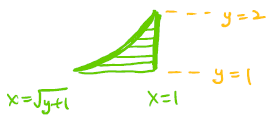
\includegraphics[width=0.75\textwidth]{iint_eg2_x_div1}
        \end{minipage}
        %
        $\displaystyle I_1 = \int_{y=1}^{y=2}\int_{x=\sqrt{y+1}}^{x=1} f(x,y) \dd{x}\dd{y}$
    \end{center}

    \begin{center}
        \begin{minipage}{0.35\textwidth}
            \centering
            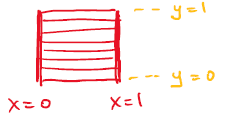
\includegraphics[width=0.7\textwidth]{iint_eg2_x_div2}
        \end{minipage}
        %
        $\displaystyle I_2 = \int_{y=0}^{y=1}\int_{x=0}^{x=1} f(x,y) \dd{x}\dd{y}$
    \end{center}
        
    \begin{center}
        \begin{minipage}{0.35\textwidth}
            \centering
            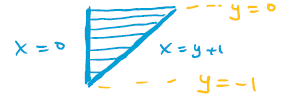
\includegraphics[width=0.78\textwidth]{iint_eg2_x_div3}
        \end{minipage}
        %
        $\displaystyle I_3 = \int_{y=0}^{y=-1}\int_{x=0}^{x=y+1} f(x,y) \dd{x}\dd{y}$
    \end{center}    


    And the final answer would be the sum to all 3 regions $I_1+I_2+I_3$. 
    Although we should get the same value as we integrate $y$ first then $x$,
    integrating $x$ first then $y$ takes a lot more effort.

\end{example}

%%%
\theend
\end{document}